\chapter{Caracterización del  Electroimán} \chapterlabel{Informe/3-CaracterizaciónElectroimán} \label{cap:CaracterizaciónElectroimán}

\section{Caracterización del Electroimán}

El actuador de este sistema de control es un electroimán. Se eligió construirlo utilizando un núcleo de acero al silicio con un bobinado en su interior. 
%mejorar esto

Se puede modelar el problema como un objeto de masa puntual que es sometido a dos fuerzas opuestas en el eje “Y” de la figura \ref{fig:img_modelado-fisico}: la de su propio peso hacia abajo, y una fuerza realizada por el electroimán en sentido contrario.

%capaz poner otra imagen
\begin{figure}[H]
	\centering
	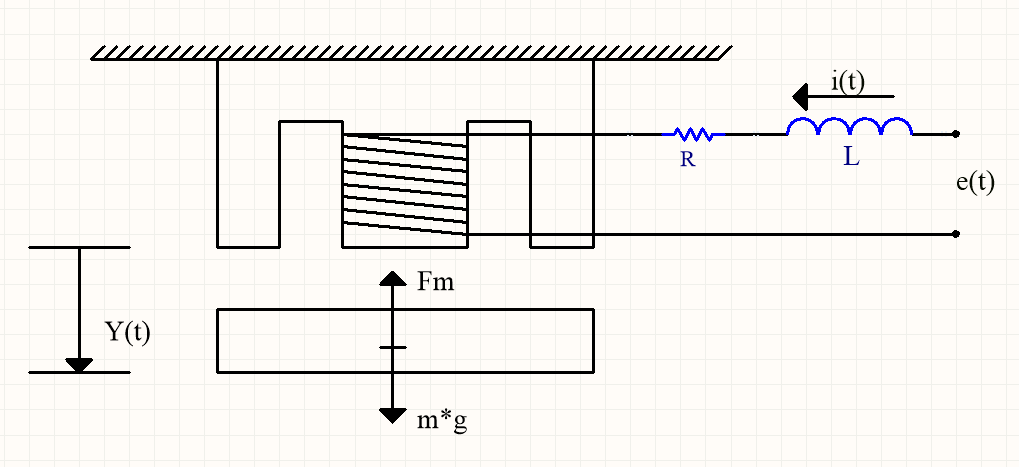
\includegraphics[width=\textwidth]{modelo-fisico.png}
	\caption{Modelado físico.}
	\label{fig:img_modelado-fisico}
\end{figure}

Se sabe que la fuerza correspondiente al peso del objeto es $F_{m}=m*g$. Por lo tanto, el electroimán debe generar una fuerza de igual módulo y sentido contrario para mantenerlo suspendido en estado de equilibrio. Esta fuerza se obtiene de la circulación de un flujo magnético entre el núcleo del electroimán y la pieza con forma de I. Para generar el flujo magnético se necesita una fuerza magnetomotriz.

%esto es otra cosa ya. hacer una intro de como se genera la fuerza magnética???
La fuerza magnetomotriz generada en el núcleo del electroimán es proporcional a la corriente que circula por su bobinado, y su módulo está dado por la ecuación \ref{eq_fuerza-magnetomotriz}. Para poder modelarla se debe realizar un análisis físico del actuador. 

\begin{equation} \label{eq_fuerza-magnetomotriz}
	F_{mm}=R_{m}*\phi=N*i	
\end{equation}

%mejorar este parrafo
En donde $R_{m}$ corresponde a la reluctancia del circuito magnético, $\phi$ indica la magnitud del flujo, es decir, la cantidad de campo magnético que atravies una superficie y $F_{mm}$ es la fuerza magnetomotriz (que es distinta a la fuerza magnética $F_{m}$). La ley de Hopkinson relaciona estos parámetros con la corriente que circula por el bobinado ($i$) y la cantidad de vueltas de su núcleo ($N$).


Por otro lado, la inductancia del bobinado está dada por la ecuación \ref{eq_inductancia_flujo}

\begin{equation} \label{eq_inductancia_flujo}
	L*i=N*\phi
\end{equation}


Como se ve en la figura \ref{fig:img_modelado-fisico}, el electroimán utilizado está compuesto por una pieza en forma de E y otra en forma de I, que se encuentran separadas por un espacio o gap de aire. Este circuito magnético se puede modelar como a un toroide con un corte o separación  de longitud $lA=2*y$, como se muestra en la figura \ref{fig:img_toroide}

\begin{figure}[H]
	\centering
	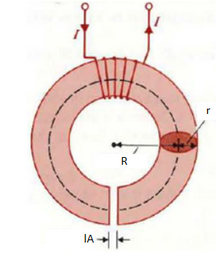
\includegraphics[scale=0.75]{toroide.png}
	\caption{Toroide con gap de aire.}
	\label{fig:img_toroide}
\end{figure}

Para el análisis se utiliza la ecuación \ref{eq_reluctancia} para modelar la reluctancia de un toroide sin gap de aire, con área transversal A, permeabilidad del material $\mu_{r}$ y longitud del circuito magnético $l_{h}$. 

\begin{equation}\label{eq_reluctancia}
	R_{m}=\frac{l_{h}}{\mu_{o}*\mu_{r}*A}
\end{equation}

Combinando las ecuaciones \ref{eq_fuerza-magnetomotriz}, \ref{eq_inductancia_flujo}, y \ref{eq_reluctancia}, se llega a la expresión de la inductancia del toroide:

\begin{equation}\label{eq_inductancia}
	L=\frac{N}{i}*\phi=\frac{N}{i}*\frac{N*i}{R_{m}}=\frac{N^	{2}*A*\mu_{o}*\mu_{r}}{l_{h}}
\end{equation}


Al agregar un gap de aire, se genera una discontinuidad en el medio magnético. Es decir, se genera una discontinuidad de distancia $l_{A}$ (longitud en el aire).

Según Maxwell, las líneas de flujo magnético son todas continuas. Es decir, no hay carga magnética como tal, a diferencia de los campos electrostáticos que sí los hay. Por lo tanto, el mismo flujo que circula por el material ferromagnético, es el que  está en el aire. 

Es posible que las líneas de flujo presentes en el gap de aire sufran de ensanchamiento provocando que las mismas no se mantengan constantes (efecto fringing). A efectos prácticos esto es despreciable ya que esta distancia es lo suficientemente pequeña dejando como sección transversal aproximada A.

Considerando que al haber un gap de aire, la reluctancia del sistema aumenta, por lo que se debe sumar, en serie a $R_{m}$, la reluctancia en el aire $R_{a}$. Por otro lado, $l_{h}$ prácticamente no se ve modificada ya que es una pequeña incisión en el flujo magnético. De esta forma, se obtiene la ecuación \ref{eq_inductancia_con_gap}.

\begin{equation}\label{eq_inductancia_con_gap}
L=\frac{N^{2}}{R_{m}*R_{a}}=\frac{N^{2}}{\frac{l_{h}}{A*\mu_{o}*\mu_{r}}+\frac{l_{a}}{A*\mu_{o}}}=\frac{N^{2}*A*\mu_{o}}{l_{a}+\frac{l_{h}}{\mu_{r}}}
\end{equation}

Sabiendo que $l_{a}$ es el gap de aire, se debe reemplazar por la distancia de separación entre las dos piezas magnéticas, la cual está representada por la variable y. En el caso de nuestro electroimán, las líneas de fuerza atraviesan dos veces y, por lo tanto $l_{a}=2*y$.

Además, considerando que en la ecuación \ref{eq_inductancia_con_gap} $\mu_{r}>>1$ entonces $2*y>>\frac{l_{h}}{\mu_{r}}$ y se obtiene la inductancia en función de la distancia del gap de aire y:

\begin{equation}\label{eq_inductancia_vs_y}
		L(y)=\frac{{N^{2}*A*\mu_{o}}}{2*y}
\end{equation}

\section{Cálculo de la fuerza magnética}

La fuerza magnética necesaria para mantener a un objeto en suspensión se puede encontrar a partir de la energía almacenada en un inductor y al considerar que esta es  igual al trabajo:

\begin{equation}\label{eq_energia}
	E(i,y)=W=\int{F_{m}*dy}=>F_{m}=\frac{\partial{E(i,y)}}{\partial{y}}
\end{equation}

Y sabiendo la expresión para obtener la energía que almacena un inductor en su campo magnético:

\begin{equation}\label{eq_energia_2}
	E(i,y)=\frac{L(i,y)*i^{2}}{2}
\end{equation}

Esto significa que la cantidad de energía que almacena el sistema es función del gap de aire. Combinando las ecuaciones \ref{eq_inductancia_vs_y}, \ref{eq_energia} y \ref{eq_energia_2}:

\begin{equation}\label{eq_fuerza_magnetica}
	\abs{F_{m}}=\frac{\partial{E(i,y)}}{\partial{y}}=\frac{i^{2}}{2}*\frac{\partial{\frac{{N^{2}*A*\mu_{o}}}{2*y}}}{\partial{y}}=\frac{i^{2}*N^{2}*\mu_{o}*A}{4*y^{2}}
\end{equation}

Como se puede apreciar en la ecuación \ref{eq_fuerza_magnetica} la fuerza es proporcional al cuadrado de la acción de control (es decir, de la corriente), e inversamente proporcional al cuadrado de la variable que se desea controlar (es decir, de la distancia). Por lo tanto, el problema adquiere un comportamiento sumamente alineal.

\section{Diseño del electroimán}

%¿sería conveniente hacer el diseño partiendo del electroimán que ya tenemos, y en base a eso determinar el peso que podemos levantar?
Se debe determinar qué dimensiones debe tener el electroimán a utilizar para que sea capaz de ejercer la fuerza magnética necesaria para mantener levitando el peso deseado.

Al analizar la ecuación \ref{eq_fuerza_magnetica} se puede observar que hay dos parámetros que son propios del electroimán: el área del núcleo A y la cantidad de vueltas del bobinado N. Para obtener una expresión de diseño, partimos de esta ecuación y la igualamos al fuerza ejercida por el peso que debe soportar ($\abs{F_{m}}=m*g$):

\begin{equation}\label{eq_fuerza_peso}
	m*g=\frac{i^{2}*N^{2}*\mu_{o}*A}{4*y^{2}}
\end{equation}

De la ecuación \ref{eq_fuerza_peso} podemos despejar el producto $N*i$ que es la fuerza magnetomotriz:

\begin{equation} \label{eq_n_por_i}
	N*i=y*\sqrt{\frac{4*m*g}{\mu_{o}*A}}
\end{equation}

Partiendo de la ecuación \ref{eq_inductancia_flujo}, reemplazando $\phi=B*A$ y considerando el caso de máxima inducción magnética ($i_{max}$):

\begin{equation}\label{eq_inductancia_densidad}
	L*i_{max}=N*B_{max}*A
\end{equation}

Luego, relacionando la ecuación \ref{eq_inductancia_vs_y} y \ref{eq_inductancia_densidad}:

\begin{equation} \label{eq_bmax}
	B_{max}=\mu_{o}*\frac{N*i_{max}}{2*y}
\end{equation}

Combinando la ecuación \ref{eq_bmax} y \ref{eq_n_por_i}:

\begin{equation}
	B_{max}=\sqrt{\frac{m*g*\mu_{o}}{A}}
\end{equation}

Finalmente:

\begin{equation} \label{eq_area}
	A>=\frac{m*g*\mu_{o}}{B_{max}^{2}}
\end{equation}

a

a
a
a


En la Figura 3.1 se puede observar una representación física del problema.


A partir del modelado físico del electroimán se llega a la expresión de la inductancia (L) en función del gap de aire (Y) (ecuación 3.1) y de la fuerza magnética ejercida por el electroimán (Fm) (ecuación 3.2):


